% MCA-report.tex - IEEE-format project report.
% Build:  cd project-report && tectonic MCA-report.tex      (or: pdflatex MCA-report.tex, twice)
\documentclass[conference]{IEEEtran}
\IEEEoverridecommandlockouts
\usepackage{cite}
\usepackage{amsmath}
\usepackage{iftex}
\ifTUTeX   % XeLaTeX / LuaLaTeX (e.g. tectonic): Times-style text and a real monospace font
  \usepackage{fontspec}
  \setmainfont{texgyretermes}[Extension=.otf, UprightFont=*-regular, BoldFont=*-bold, ItalicFont=*-italic, BoldItalicFont=*-bolditalic]
  \setmonofont{lmmono10}[Extension=.otf, UprightFont=*-regular, ItalicFont=*-italic, BoldFont=lmmonolt10-bold, Scale=0.98]
\else      % pdfLaTeX
  \usepackage[T1]{fontenc}
  \usepackage{newtxtext,newtxmath}
\fi
\usepackage{graphicx}
\usepackage{booktabs}
\usepackage{array}
\usepackage{listings}
\usepackage[table]{xcolor}
\usepackage{xurl}
\usepackage[hidelinks]{hyperref}
\graphicspath{{figures/}{../docs/logisim/}}

\definecolor{codebg}{RGB}{246,248,252}
\lstset{basicstyle=\ttfamily\scriptsize, backgroundcolor=\color{codebg}, frame=single, rulecolor=\color{black!25},
  columns=fullflexible, keepspaces=true, breaklines=true, xleftmargin=2pt, xrightmargin=2pt, aboveskip=6pt, belowskip=4pt}

\newcommand{\repo}{https://github.com/khushi-madan18/Single-Cycle-MIPS-Processor-with-Memory-Interface}
\newcommand{\live}{https://khushi-madan18.github.io/Single-Cycle-MIPS-Processor-with-Memory-Interface/}

% start a new row of authors in the IEEEtran author block
\makeatletter
\newcommand{\linebreakand}{\end{@IEEEauthorhalign}\hfill\mbox{}\par\mbox{}\hfill\begin{@IEEEauthorhalign}}
\makeatother

\begin{document}

\title{Design, Simulation and Verification of a 32-bit\\Single-Cycle MIPS Processor with Memory Interface}

\author{
\IEEEauthorblockN{Avneet Singh}
\IEEEauthorblockA{Enrollment No. 2401010117}
\and
\IEEEauthorblockN{Khushi}
\IEEEauthorblockA{Enrollment No. 2401010225}
\and
\IEEEauthorblockN{Manpreet Singh}
\IEEEauthorblockA{Enrollment No. 2401010263}
\linebreakand
\IEEEauthorblockN{Riya Yadav}
\IEEEauthorblockA{Enrollment No. 2401010390}
\and
\IEEEauthorblockN{Satvik Prasad}
\IEEEauthorblockA{Enrollment No. 2401020055}
}

\maketitle

\begin{abstract}
This paper presents a 32-bit single-cycle MIPS processor implemented in Verilog-2001. The processor supports a MIPS32 subset: R-type ADD, SUB, AND, OR and SLT; ADDI; word load and store (LW and SW); conditional branch (BEQ); and jump (J). The datapath and control logic form a reusable core that is connected to separate instruction and data memories through explicit interfaces. The design is verified with Icarus Verilog testbenches at three levels: unit testbenches for the ALU and the control unit, a self-checking system testbench, and a program testbench that runs four assembly programs and dumps VCD waveforms. Every simulated clock cycle is compared with an independent Python golden model. The full regression passes 9/9 checks, and the RTL, the golden model, a Logisim-evolution circuit and a browser-based simulator agree on all 265 clock cycles of the sample programs. The paper describes the architecture, the testbench environment, waveform analysis of the instruction flow, Yosys synthesis results and the limitations of the single-cycle organization.
\end{abstract}

\begin{IEEEkeywords}
MIPS32, single-cycle processor, Verilog, testbench, simulation waveform, datapath, control unit, memory interface, RTL verification, synthesis.
\end{IEEEkeywords}

\section{Introduction}
A processor executes a program by repeatedly fetching an instruction, decoding its fields, reading operands, performing an operation, accessing memory when required and updating architectural state. The objective of this project is to implement these functions as connected digital hardware, to study the relationship between datapath components and control signals, and to show through simulation that the hardware behaves correctly on every clock cycle.

The design uses a single-cycle organization: every supported instruction completes in one clock period. Instruction fetch, decode, execution, memory access and write-back are combinationally connected between state elements, and only the program counter, the register-file write port and the data-memory write port update on clock edges. This structure suits learning because the complete instruction path can be traced within one cycle. Its main drawback is that the clock period must accommodate the slowest instruction.

The implementation separates the processor core from the memories. The \texttt{mips\_core} module contains the datapath and control logic, while \texttt{mips\_cpu} connects the core to instruction and data memories. This explicit interface makes the core reusable with other memory implementations and allows the core to be synthesized independently of the program image.

The objectives of this work are: (i) to implement a 32-bit single-cycle MIPS core in Verilog-2001~\cite{verilog} for a defined instruction subset; (ii) to separate the core from the instruction and data memories through explicit interfaces; (iii) to verify the design with testbenches at component, system and program level, and to analyse its behaviour with simulation waveforms; and (iv) to document its synthesis footprint and the timing cost of the single-cycle organization.

The source code, testbenches, waveforms and this report are available at \url{\repo}. The interactive simulator runs at \url{\live}.

\section{Related Work}
The MIPS architecture is the standard teaching example for processor design, and the single-cycle, multi-cycle and pipelined organizations are described in detail by Patterson and Hennessy~\cite{patterson}. The instruction set itself is defined in the MIPS32 architecture manual~\cite{mips32}. Many HDL implementations of 32-bit MIPS-style processors have been published, and most of them target pipelined organizations.

Bhardwaj~\cite{bhardwaj} presents the design and simulation of a five-stage pipelined 32-bit MIPS processor in Verilog, simulated in ModelSim, with RTL design carried out using Xilinx tools. Phanindra~\cite{phanindra} reports another 32-bit MIPS-based RISC processor design. At larger scale, Al-Sudany et al.~\cite{alsudany} build a pipelined MIPS processor in VHDL with a datapath, a control unit and a hazard unit. It resolves data, control and structural hazards, is replicated into four SIMD pipelined cores and is implemented on a Xilinx Virtex-6 FPGA, with a reported power of 3.422~W and a clock period of 7.329~ns.

These works concentrate on pipelining, hazard handling, FPGA implementation and performance. The present project has a different emphasis. It keeps the simpler single-cycle organization so that the whole instruction path can be traced within one clock period, and places weight on verification and reproducibility: separate core and memory modules, self-checking testbenches, cycle-by-cycle comparison with a Python golden model, waveform analysis, a Logisim circuit checked against the Verilog trace, and a Yosys synthesis flow~\cite{yosys}. The pipelined designs above also show why the single-cycle critical path discussed in Section~\ref{sec:synth} is worth measuring, since pipelining is the usual way to shorten it.

\section{Background and Design Approach}
The classical single-cycle MIPS datapath~\cite{patterson} combines a program counter, instruction memory, register file, ALU, data memory, multiplexers and control logic. The instruction opcode selects the broad operation and determines which resources are enabled. R-type operations additionally use the function field to select an ALU operation.

R-type fields identify two source registers, a destination register, a shift amount and a function code. I-type instructions contain a 16-bit immediate used for arithmetic, memory displacement or branch offset. J-type instructions contain a 26-bit target. The implemented subset (Table~\ref{tab:isa}) is intentionally limited and is not a complete MIPS32 implementation.

\begin{table}[t]
\caption{Supported Instructions}
\label{tab:isa}
\centering\footnotesize\setlength{\tabcolsep}{4pt}
\begin{tabular}{@{}lll@{}}
\toprule
Instruction & Format & Function\\
\midrule
ADD, SUB, AND, OR, SLT & R-type & Register arithmetic/logic\\
ADDI & I-type & Add sign-extended immediate\\
LW & I-type & Load word from data memory\\
SW & I-type & Store word to data memory\\
BEQ & I-type & Branch if registers are equal\\
J & J-type & Unconditional jump\\
\bottomrule
\end{tabular}
\end{table}

\section{System Architecture}
\subsection{Top-Level Organization}
The \texttt{mips\_core} module contains the PC, instruction decode, main control unit, register file, sign-extension unit, ALU control, ALU, write-back selection and branch/jump logic. The top-level \texttt{mips\_cpu} module instantiates the core, the instruction memory and the data memory, giving a Harvard-style organization. The core outputs an instruction byte address and receives a 32-bit instruction word; it also outputs a data address, store data and memory read/write enables, and receives loaded data. Fig.~\ref{fig:logisim} shows the datapath as modelled in Logisim-evolution~\cite{logisim}.

\begin{figure}[t]
\centering
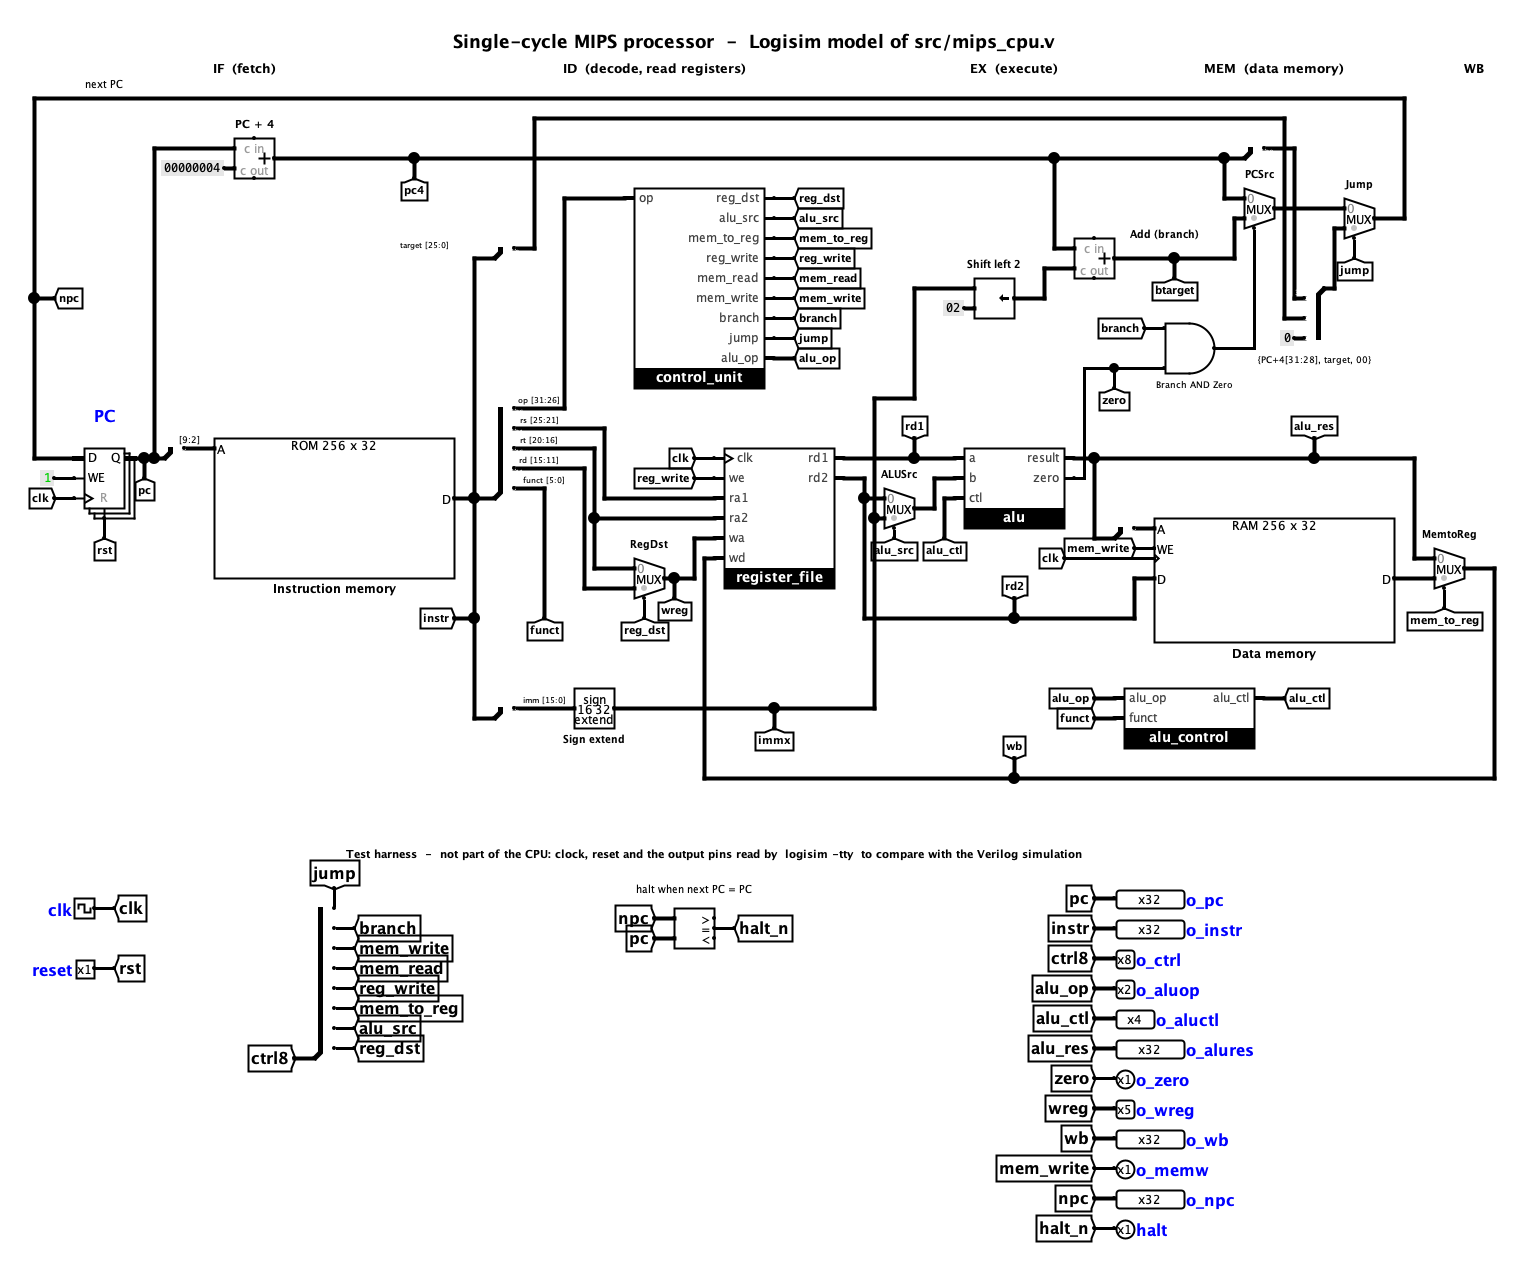
\includegraphics[width=\columnwidth]{main.png}
\caption{Logisim-evolution datapath of the processor. The circuit is checked against the Verilog simulation on every clock cycle.}
\label{fig:logisim}
\end{figure}

\subsection{Datapath Components}
\emph{Program counter:} a 32-bit register holding the current byte address. Sequential execution selects PC+4; branch and jump logic can override this value. Reset is synchronous and active-high.

\emph{Instruction memory:} a 256-word by 32-bit ROM-style array with a combinational read port, initialized from a hexadecimal image produced by the assembler.

\emph{Register file:} 32 registers of 32 bits with two asynchronous read ports and one synchronous write port. Register \$zero always reads as zero and ignores writes.

\emph{Sign extension and ALU:} the sign-extension unit replicates bit 15 of the immediate to form a 32-bit operand. The ALU performs addition, subtraction, bitwise AND, bitwise OR and signed set-less-than. Its zero output is asserted when the result is zero, which lets BEQ test equality.

\emph{Data memory:} a 256-word by 32-bit RAM with combinational reads gated by MemRead and synchronous writes gated by MemWrite. Accesses are word-aligned: address bits [9:2] select the word and the low two bits are ignored.

\subsection{Core-to-Memory Interface}
The instruction interface consists of \texttt{imem\_addr} and \texttt{imem\_rdata}. The data interface consists of \texttt{dmem\_addr}, \texttt{dmem\_wdata}, \texttt{dmem\_we}, \texttt{dmem\_re} and \texttt{dmem\_rdata}. For LW and SW the ALU computes the effective byte address as a base register plus a sign-extended displacement, and the store-data bus carries the second register operand. The same core can therefore be attached to simulation memories or to other compatible memory blocks.

\section{Instruction Set and Control}
\subsection{Main Control Unit}
The control unit decodes the 6-bit opcode and generates RegDst, ALUSrc, MemtoReg, RegWrite, MemRead, MemWrite, Branch, Jump and ALUOp (Table~\ref{tab:ctrl}). RegDst selects rd (R-type) or rt (I-type) as the destination register; ALUSrc selects a register or the sign-extended immediate as the second ALU operand; MemtoReg chooses the ALU result or memory data for write-back; RegWrite enables register updates; MemRead and MemWrite control the data memory; Branch and Jump control next-PC selection. Unused control values are driven to zero, so an unknown opcode behaves as a no-operation.

The ALU-control block combines ALUOp with the R-type function field: ALUOp=00 selects addition (ADDI, LW, SW), ALUOp=01 selects subtraction (BEQ), and ALUOp=10 lets the function field select ADD, SUB, AND, OR or SLT.

\begin{table}[t]
\caption{Main Control Signals per Instruction}
\label{tab:ctrl}
\centering\footnotesize\setlength{\tabcolsep}{4.2pt}
\begin{tabular}{@{}lccccccccc@{}}
\toprule
Instr. & RD & AS & M2R & RW & MR & MW & Br & J & ALUOp\\
\midrule
R-type & 1 & 0 & 0 & 1 & 0 & 0 & 0 & 0 & 10\\
LW     & 0 & 1 & 1 & 1 & 1 & 0 & 0 & 0 & 00\\
SW     & 0 & 1 & 0 & 0 & 0 & 1 & 0 & 0 & 00\\
BEQ    & 0 & 0 & 0 & 0 & 0 & 0 & 1 & 0 & 01\\
ADDI   & 0 & 1 & 0 & 1 & 0 & 0 & 0 & 0 & 00\\
J      & 0 & 0 & 0 & 0 & 0 & 0 & 0 & 1 & 00\\
\bottomrule
\multicolumn{10}{@{}p{0.95\columnwidth}@{}}{\scriptsize RD = RegDst, AS = ALUSrc, M2R = MemtoReg, RW = RegWrite, MR = MemRead, MW = MemWrite, Br = Branch, J = Jump.}
\end{tabular}
\end{table}

\subsection{Next-PC Logic}
The sequential address is PC+4. The branch target is PC+4 plus the sign-extended immediate shifted left by two. The jump target concatenates the upper four bits of PC+4, the 26-bit jump field and two zero bits. The next PC is the jump target when Jump is asserted, otherwise the branch target when Branch AND Zero is true, otherwise PC+4. This keeps instruction addresses word-aligned and follows standard MIPS address formation~\cite{mips32}.

\section{Assembly and Execution Flow}
Assembly programs are stored in the \texttt{programs} directory. A two-pass assembler resolves labels and register names, supports \texttt{.data} and \texttt{.word} declarations, and generates a hexadecimal instruction image (\texttt{.mem}), a data image and a conversion listing (\texttt{.lst}). The testbench loads these images into the memories with \texttt{\$readmemh}. A program terminates with a self-jump (\texttt{halt: j halt}); the program testbench detects the halt when the next PC equals the current PC.

The project also includes an interactive browser-based simulator (Fig.~\ref{fig:ui}). It shows the assembly-to-machine-code conversion, an animated datapath, control signals, registers and memory, the recorded testbench results and the VCD waveforms, and it compares every cycle it executes with the Verilog simulation trace.

\begin{figure}[t]
\centering
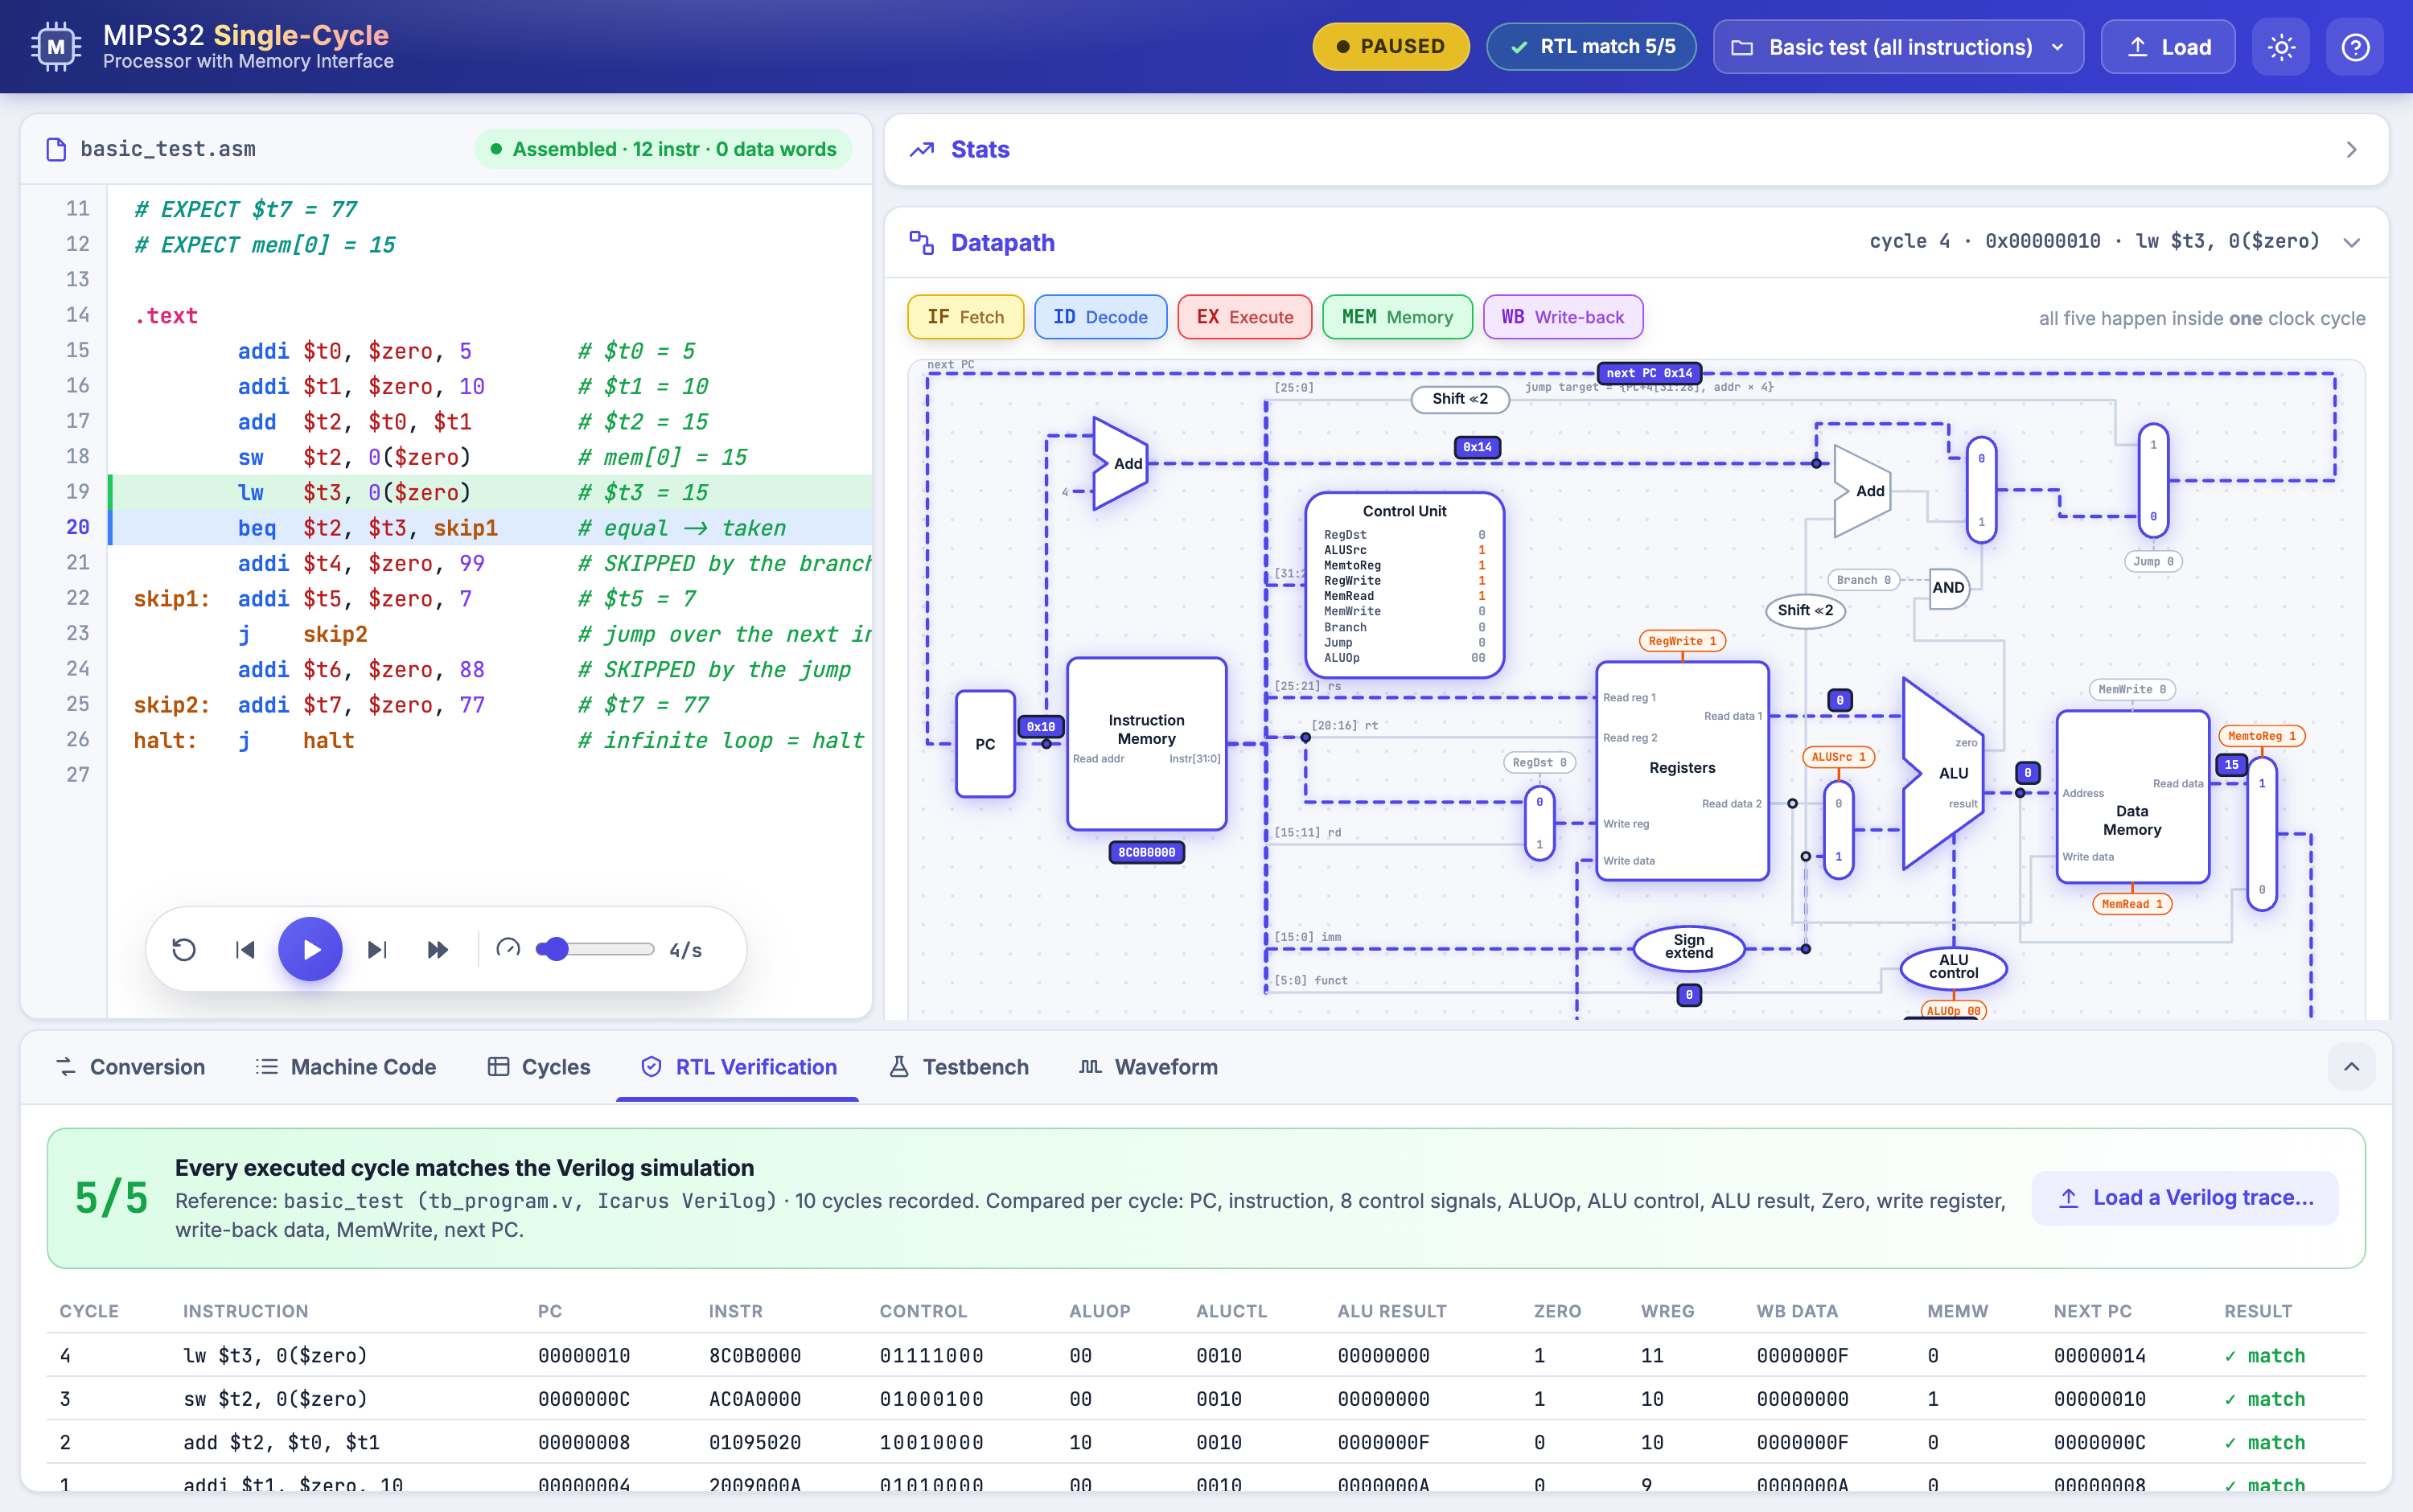
\includegraphics[width=\columnwidth]{simulator.png}
\caption{Web simulator executing \texttt{lw \$t3, 0(\$zero)} in cycle 4 of \texttt{basic\_test}. The datapath shows the active path and control values; the RTL Verification tab confirms that each executed cycle matches the Verilog simulation.}
\label{fig:ui}
\end{figure}

\section{Testbench Simulation and Waveform Analysis}
\label{sec:tb}
\subsection{Simulation Environment}
All testbenches are written in Verilog-2001 and simulated with Icarus Verilog 13.0~\cite{iverilog} using \texttt{`timescale 1ns/1ps}. The system and program testbenches generate a 10~ns clock (\texttt{always \#5 clk = \textasciitilde clk}), hold reset for two rising edges, release it at 16~ns, and dump every signal of the design to a VCD file with \texttt{\$dumpfile}/\texttt{\$dumpvars}. Signals are logged at the falling clock edge, when the combinational logic of the current instruction has settled; state is updated at the next rising edge. Table~\ref{tab:tbs} lists the testbench suite and its results.

\begin{table}[t]
\caption{Testbench Suite (Icarus Verilog 13.0)}
\label{tab:tbs}
\centering\footnotesize\setlength{\tabcolsep}{3pt}
\begin{tabular}{@{}p{2.0cm}p{1.6cm}p{3.15cm}c@{}}
\toprule
Testbench & DUT & What is checked & Result\\
\midrule
\texttt{tb\_alu.v} & ALU, ALU control & 14 ALU vectors (AND, OR, ADD, SUB, signed SLT, wrap-around, zero flag) and 7 ALU-control decodes & 21/21\\
\texttt{tb\_control\_}\allowbreak\texttt{unit.v} & Control unit & all 9 control outputs for 6 opcodes and 1 unknown opcode & 7/7\\
\texttt{tb\_mips\_cpu.v} & \texttt{mips\_cpu} & self-checking run of \texttt{basic\_test}: 9 registers and \texttt{mem[0]} & 10/10\\
\texttt{tb\_program.v} $\times$4 & \texttt{mips\_cpu} & 265 cycles compared with the golden model, final 32 registers and 256 memory words, 16 \texttt{EXPECT} values & 4/4\\
\bottomrule
\end{tabular}
\end{table}

\subsection{Unit Testbenches}
\texttt{tb\_alu.v} applies fixed operand vectors to the ALU and compares both the 32-bit result and the zero flag with expected values. The vectors include overflow wrap-around (\texttt{0xFFFFFFFF + 1 = 0}), negative operands ($7 + (-3) = 4$, $3-5=-2$) and signed comparisons such as $-1 < 1$ and $\texttt{0x80000000} < \texttt{0x7FFFFFFF}$. It then checks the ALU-control decoding for every ALUOp and function code. All 21 checks pass.

\texttt{tb\_control\_unit.v} drives each opcode into the control unit and compares the nine outputs with Table~\ref{tab:ctrl}. Its console output is reproduced below; the bit order is RegDst, ALUSrc, MemtoReg, RegWrite, MemRead, MemWrite, Branch, Jump, ALUOp.
\begin{lstlisting}
Control unit test  (RegDst ALUSrc MemtoReg RegWrite MemRead MemWrite Branch Jump ALUOp)
  PASS  R-type opcode=000000  signals=1001000010
  PASS  LW     opcode=100011  signals=0111100000
  PASS  SW     opcode=101011  signals=0100010000
  PASS  BEQ    opcode=000100  signals=0000001001
  PASS  ADDI   opcode=001000  signals=0101000000
  PASS  J      opcode=000010  signals=0000000100
  PASS  unknwn opcode=111111  signals=0000000000
ALL CONTROL UNIT TESTS PASSED
\end{lstlisting}

\subsection{System Testbench}
\texttt{tb\_mips\_cpu.v} instantiates the complete \texttt{mips\_cpu} with \texttt{basic\_test}, which uses every supported instruction once. It prints PC, instruction, ALU result and next PC on every cycle and then checks the final state. An excerpt of the recorded output:
\begin{lstlisting}
cycle 0 | PC=0x00000000 | instr=0x20080005 | ALU=0x00000005 | next PC=0x00000004
cycle 3 | PC=0x0000000c | instr=0xac0a0000 | ALU=0x00000000 | next PC=0x00000010
cycle 5 | PC=0x00000014 | instr=0x114b0001 | ALU=0x00000000 | next PC=0x0000001c
cycle 7 | PC=0x00000020 | instr=0x0800000a | ALU=0x00000000 | next PC=0x00000028
...
=============== Self-Check ===============
  PASS  $t0 = 5        PASS  $t1 = 10       PASS  $t2 = 15
  PASS  $t3 = 15       PASS  $t4 = 0        PASS  $t5 = 7
  PASS  $t6 = 0        PASS  $t7 = 77       PASS  mem[0] = 15
ALL TESTS PASSED
\end{lstlisting}
\$t4 and \$t6 remain zero because the instructions that would set them are skipped by the taken branch and the jump.

\subsection{Program Testbench and Golden-Model Comparison}
\texttt{tb\_program.v} runs any assembled program until it halts, writes a per-cycle trace, the final register and memory state, and a VCD waveform. The regression script (\texttt{tools/run\_tests.py}) assembles each program, executes it on a Python golden model and compares, for every clock cycle, the PC, instruction, all control signals, ALUOp, ALU control and result, zero flag, write register, write-back data, memory-write enable and data, and next PC. It also checks that the control signals agree with Table~\ref{tab:ctrl}, compares all 32 registers and 256 data-memory words at the end, and checks the hand-computed \texttt{\# EXPECT} values in each source file. Table~\ref{tab:progs} summarises the four programs; all of them match the golden model on every cycle.

\begin{table}[t]
\caption{Program Testbench Results}
\label{tab:progs}
\centering\footnotesize\setlength{\tabcolsep}{4pt}
\begin{tabular}{@{}lccl@{}}
\toprule
Program & Instr. & Cycles & Verified result\\
\midrule
\texttt{basic\_test} & 12 & 10 & \$t7 = 77, \texttt{mem[0]} = 15\\
\texttt{array\_sum}  & 11 & 54 & sum = 110, \$t1 = 0\\
\texttt{max\_search} & 15 & 73 & maximum = 92\\
\texttt{factorial}   & 17 & 128 & 6! = 720\\
\midrule
Total & & 265 & 265/265 cycles match\\
\bottomrule
\end{tabular}
\end{table}

\subsection{Waveform Analysis}
Fig.~\ref{fig:wave1} shows the VCD waveform written by \texttt{tb\_program.v} for \texttt{basic\_test}, displayed in the waveform viewer of the web simulator. The numbers above the waveform are clock cycles; each cycle is sampled at the falling clock edge. Before the first rising edge under reset the PC and every signal derived from it are unknown (\texttt{x}), as expected for an uninitialised register; from cycle 0 onward every bus holds a defined value. Table~\ref{tab:trace} lists the same cycles from the simulation trace.

\begin{figure*}[t]
\centering
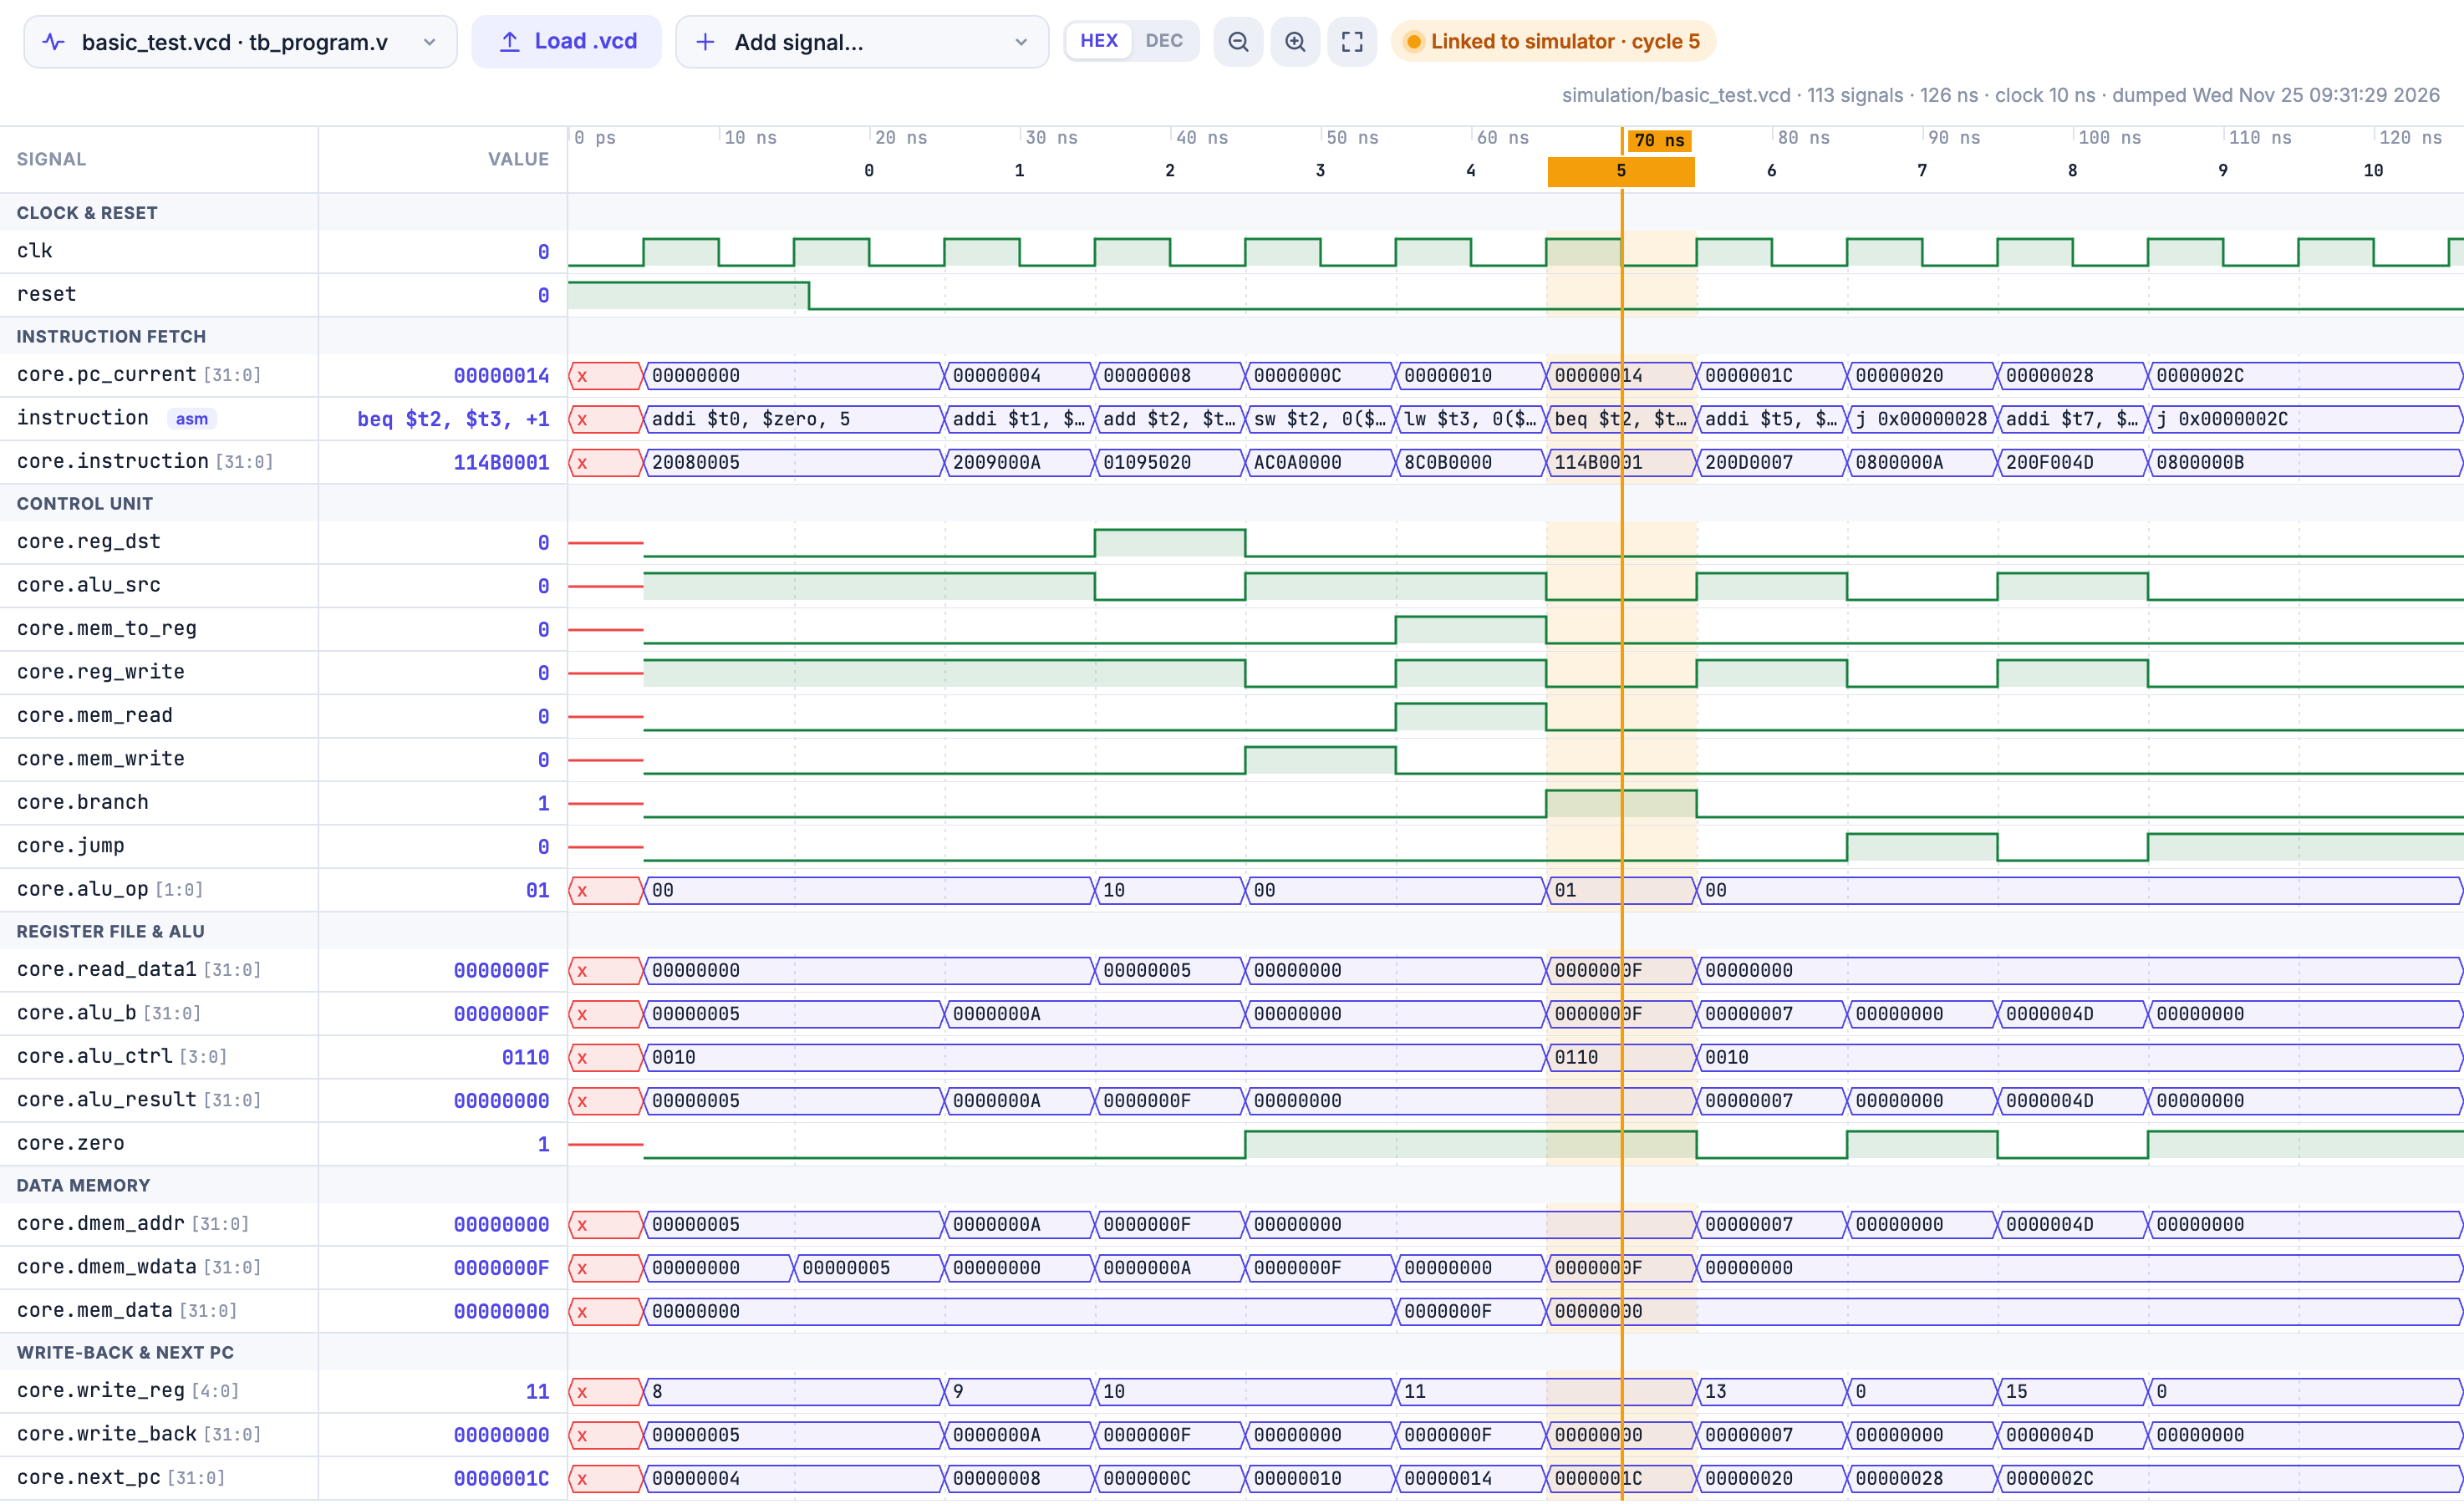
\includegraphics[width=\textwidth]{wave_basic_test.png}
\caption{Simulation waveform of \texttt{basic\_test} (VCD from \texttt{tb\_program.v}, Icarus Verilog). The cursor is on cycle 5, the taken \texttt{beq \$t2, \$t3, skip1}: Branch = 1, ALU control = 0110 (subtract), the ALU result is 0 so Zero = 1, no register or memory is written, and next\_pc jumps from 0x14 to the branch target 0x1C instead of 0x18. Cycle 3 shows the store (MemWrite = 1, store data 0x0F) and cycle 4 the load (MemRead = 1, MemtoReg = 1, memory data 0x0F written back to register 11, \$t3).}
\label{fig:wave1}
\end{figure*}

\begin{table}[t]
\caption{Simulation Trace of \texttt{basic\_test} (from \texttt{tb\_program.v})}
\label{tab:trace}
\centering\scriptsize\setlength{\tabcolsep}{2.5pt}
\begin{tabular}{@{}rllllll@{}}
\toprule
Cyc & PC & Instruction & ALU & WReg & WB data & Next PC\\
\midrule
0 & 00 & \texttt{addi \$t0,\$zero,5}  & 05 & 8  & 05 & 04\\
1 & 04 & \texttt{addi \$t1,\$zero,10} & 0A & 9  & 0A & 08\\
2 & 08 & \texttt{add \$t2,\$t0,\$t1}  & 0F & 10 & 0F & 0C\\
3 & 0C & \texttt{sw \$t2,0(\$zero)}   & 00 & -- & -- & 10\\
4 & 10 & \texttt{lw \$t3,0(\$zero)}   & 00 & 11 & 0F & 14\\
5 & 14 & \texttt{beq \$t2,\$t3,skip1} & 00 & -- & -- & 1C\\
6 & 1C & \texttt{addi \$t5,\$zero,7}  & 07 & 13 & 07 & 20\\
7 & 20 & \texttt{j skip2}             & 00 & -- & -- & 28\\
8 & 28 & \texttt{addi \$t7,\$zero,77} & 4D & 15 & 4D & 2C\\
9 & 2C & \texttt{j halt}              & 00 & -- & -- & 2C\\
\bottomrule
\end{tabular}
\end{table}

The waveform makes the single-cycle behaviour visible. Each instruction occupies exactly one clock period, and the control signals change once per cycle according to Table~\ref{tab:ctrl}. In cycle 2 (\texttt{add}) RegDst switches to 1 and ALUOp to 10, so the destination comes from the rd field. In cycle 7 the Jump signal selects the jump target 0x28 and skips \texttt{addi \$t6}. In cycle 9 next\_pc equals pc\_current (0x2C), which is the halt condition detected by the testbench.

Fig.~\ref{fig:wave2} shows cycles 2--16 of \texttt{array\_sum}, which runs a loop over eight data words. The \texttt{beq \$t1, \$zero, done} at PC 0x0C is evaluated once per iteration: the counter is non-zero, so Zero = 0 and the branch falls through to PC 0x10 (cycles 3 and 9). The \texttt{lw} at PC 0x10 reads successive array elements (12 in cycle 4, 7 in cycle 10) through the memory interface, and the \texttt{j loop} at PC 0x20 returns to 0x0C. In the last iteration the counter reaches zero, Zero becomes 1 and the branch leaves the loop, after which the sum 110 is stored.

\begin{figure*}[t]
\centering
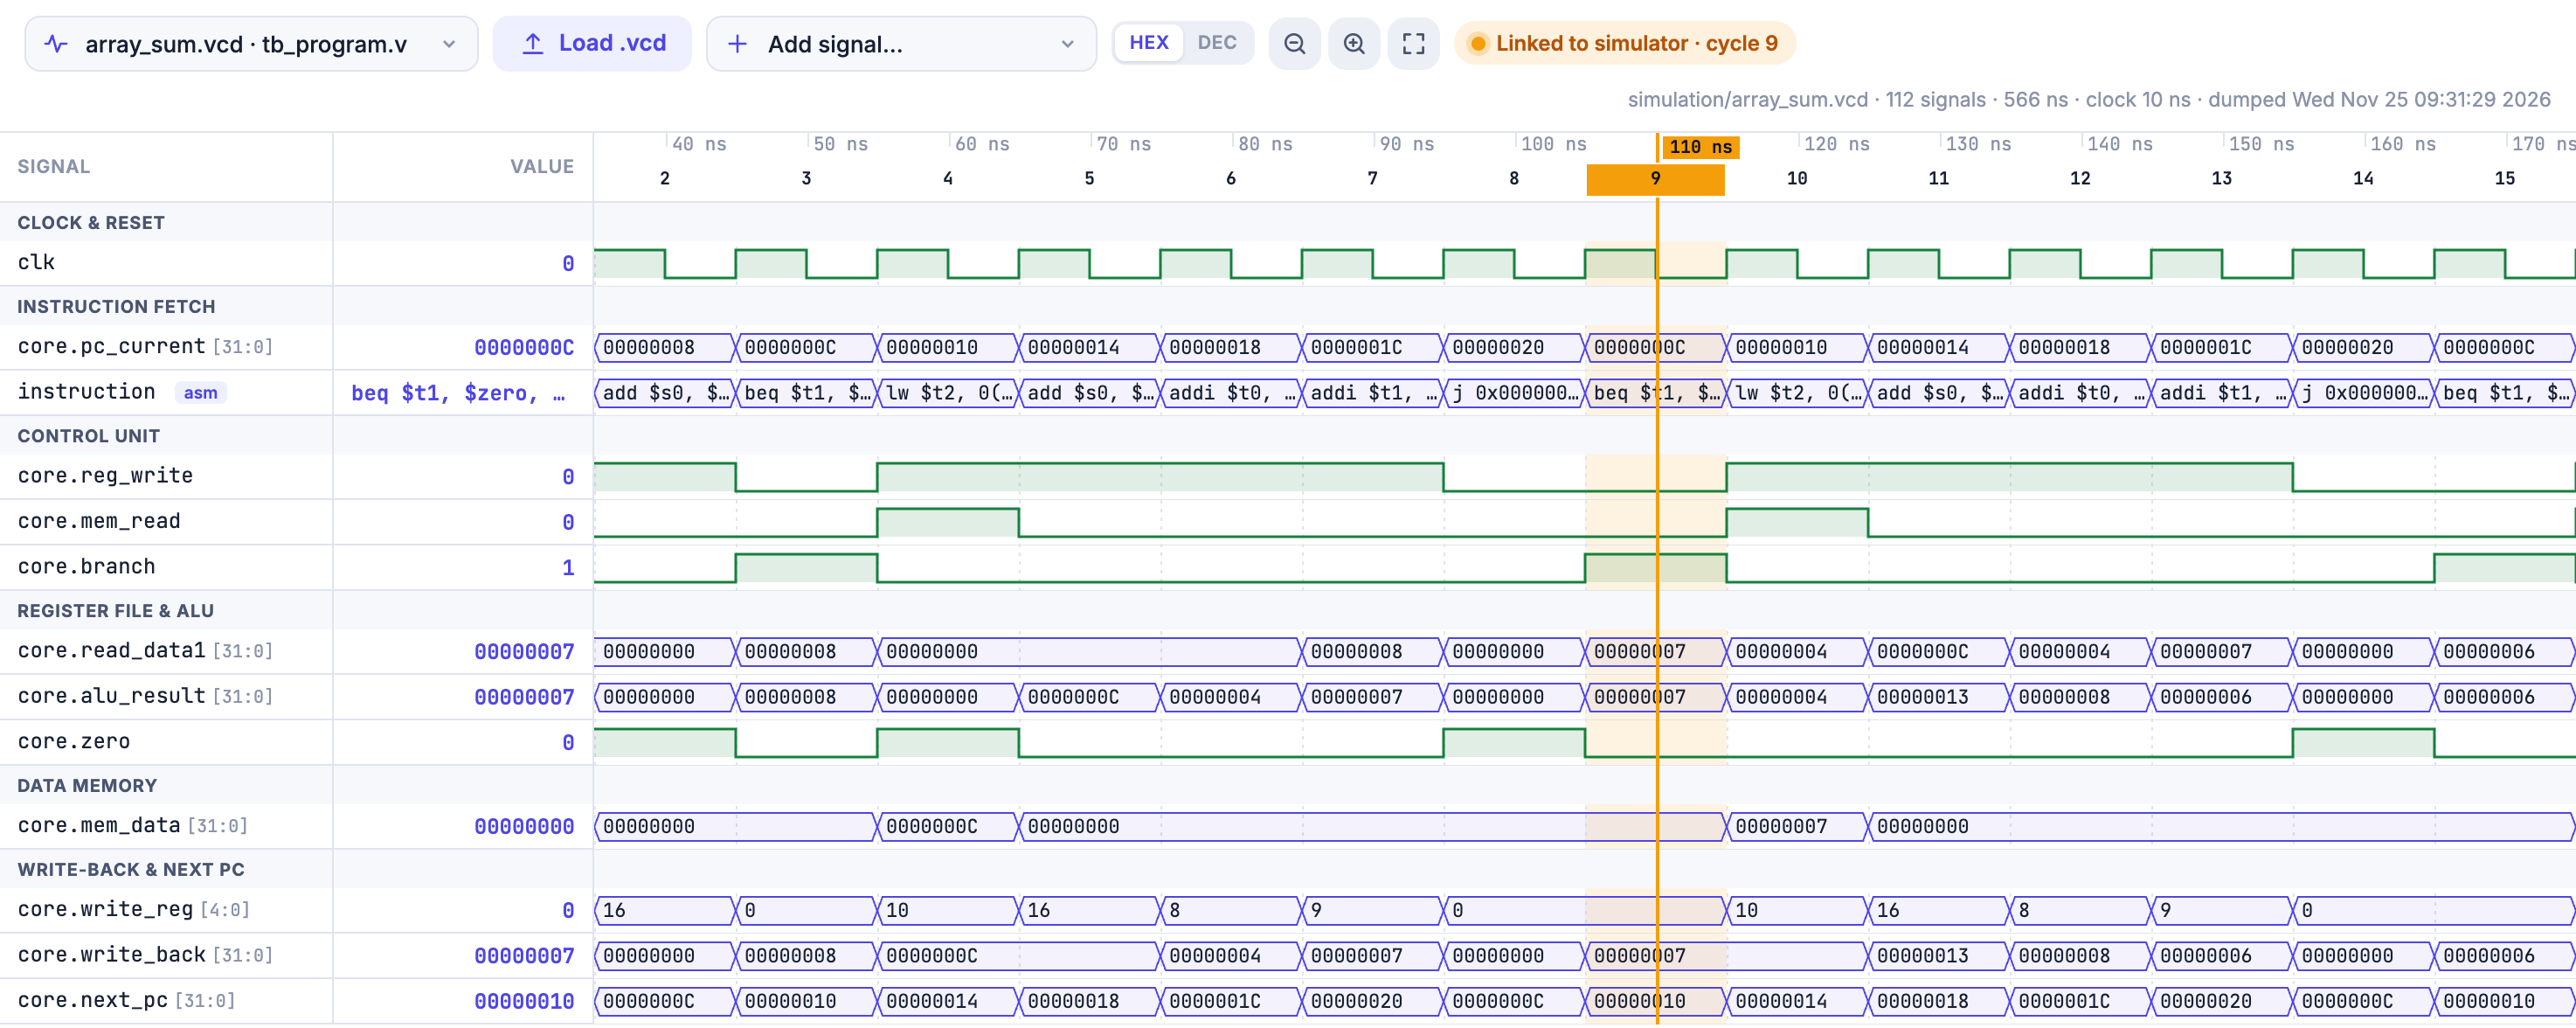
\includegraphics[width=\textwidth]{wave_array_sum.png}
\caption{Waveform of the \texttt{array\_sum} loop (cycles 2--16). The cursor is on cycle 9, a not-taken \texttt{beq \$t1, \$zero, done}: Branch = 1 but Zero = 0, so next\_pc = PC+4 = 0x10. The \texttt{lw} in the following cycle reads the second element (7) from data memory and writes it back to \$t2 (register 10).}
\label{fig:wave2}
\end{figure*}

\subsection{Regression Summary}
The complete regression is run with \texttt{make test}. Besides the Verilog testbenches it checks the web simulator's JavaScript model and the Logisim circuit against the RTL trace on every cycle. The recorded result is:
\begin{lstlisting}
PASS   tb_alu
PASS   tb_control_unit
PASS   tb_mips_cpu
PASS   programs/array_sum.asm - 11 instr, 54 cycles, 3 EXPECT checks
PASS   programs/basic_test.asm - 12 instr, 10 cycles, 9 EXPECT checks
PASS   programs/factorial.asm - 17 instr, 128 cycles, 2 EXPECT checks
PASS   programs/max_search.asm - 15 instr, 73 cycles, 2 EXPECT checks
PASS   ui/js/isa.js vs RTL (node)
PASS   logisim/mips_single_cycle.circ vs RTL
9/9 passed
\end{lstlisting}
The testbench results, console output, testbench source code and VCD waveforms are also published in the web simulator's \emph{Testbench} and \emph{Waveform} tabs (Fig.~\ref{fig:tbtab}).

\begin{figure}[t]
\centering
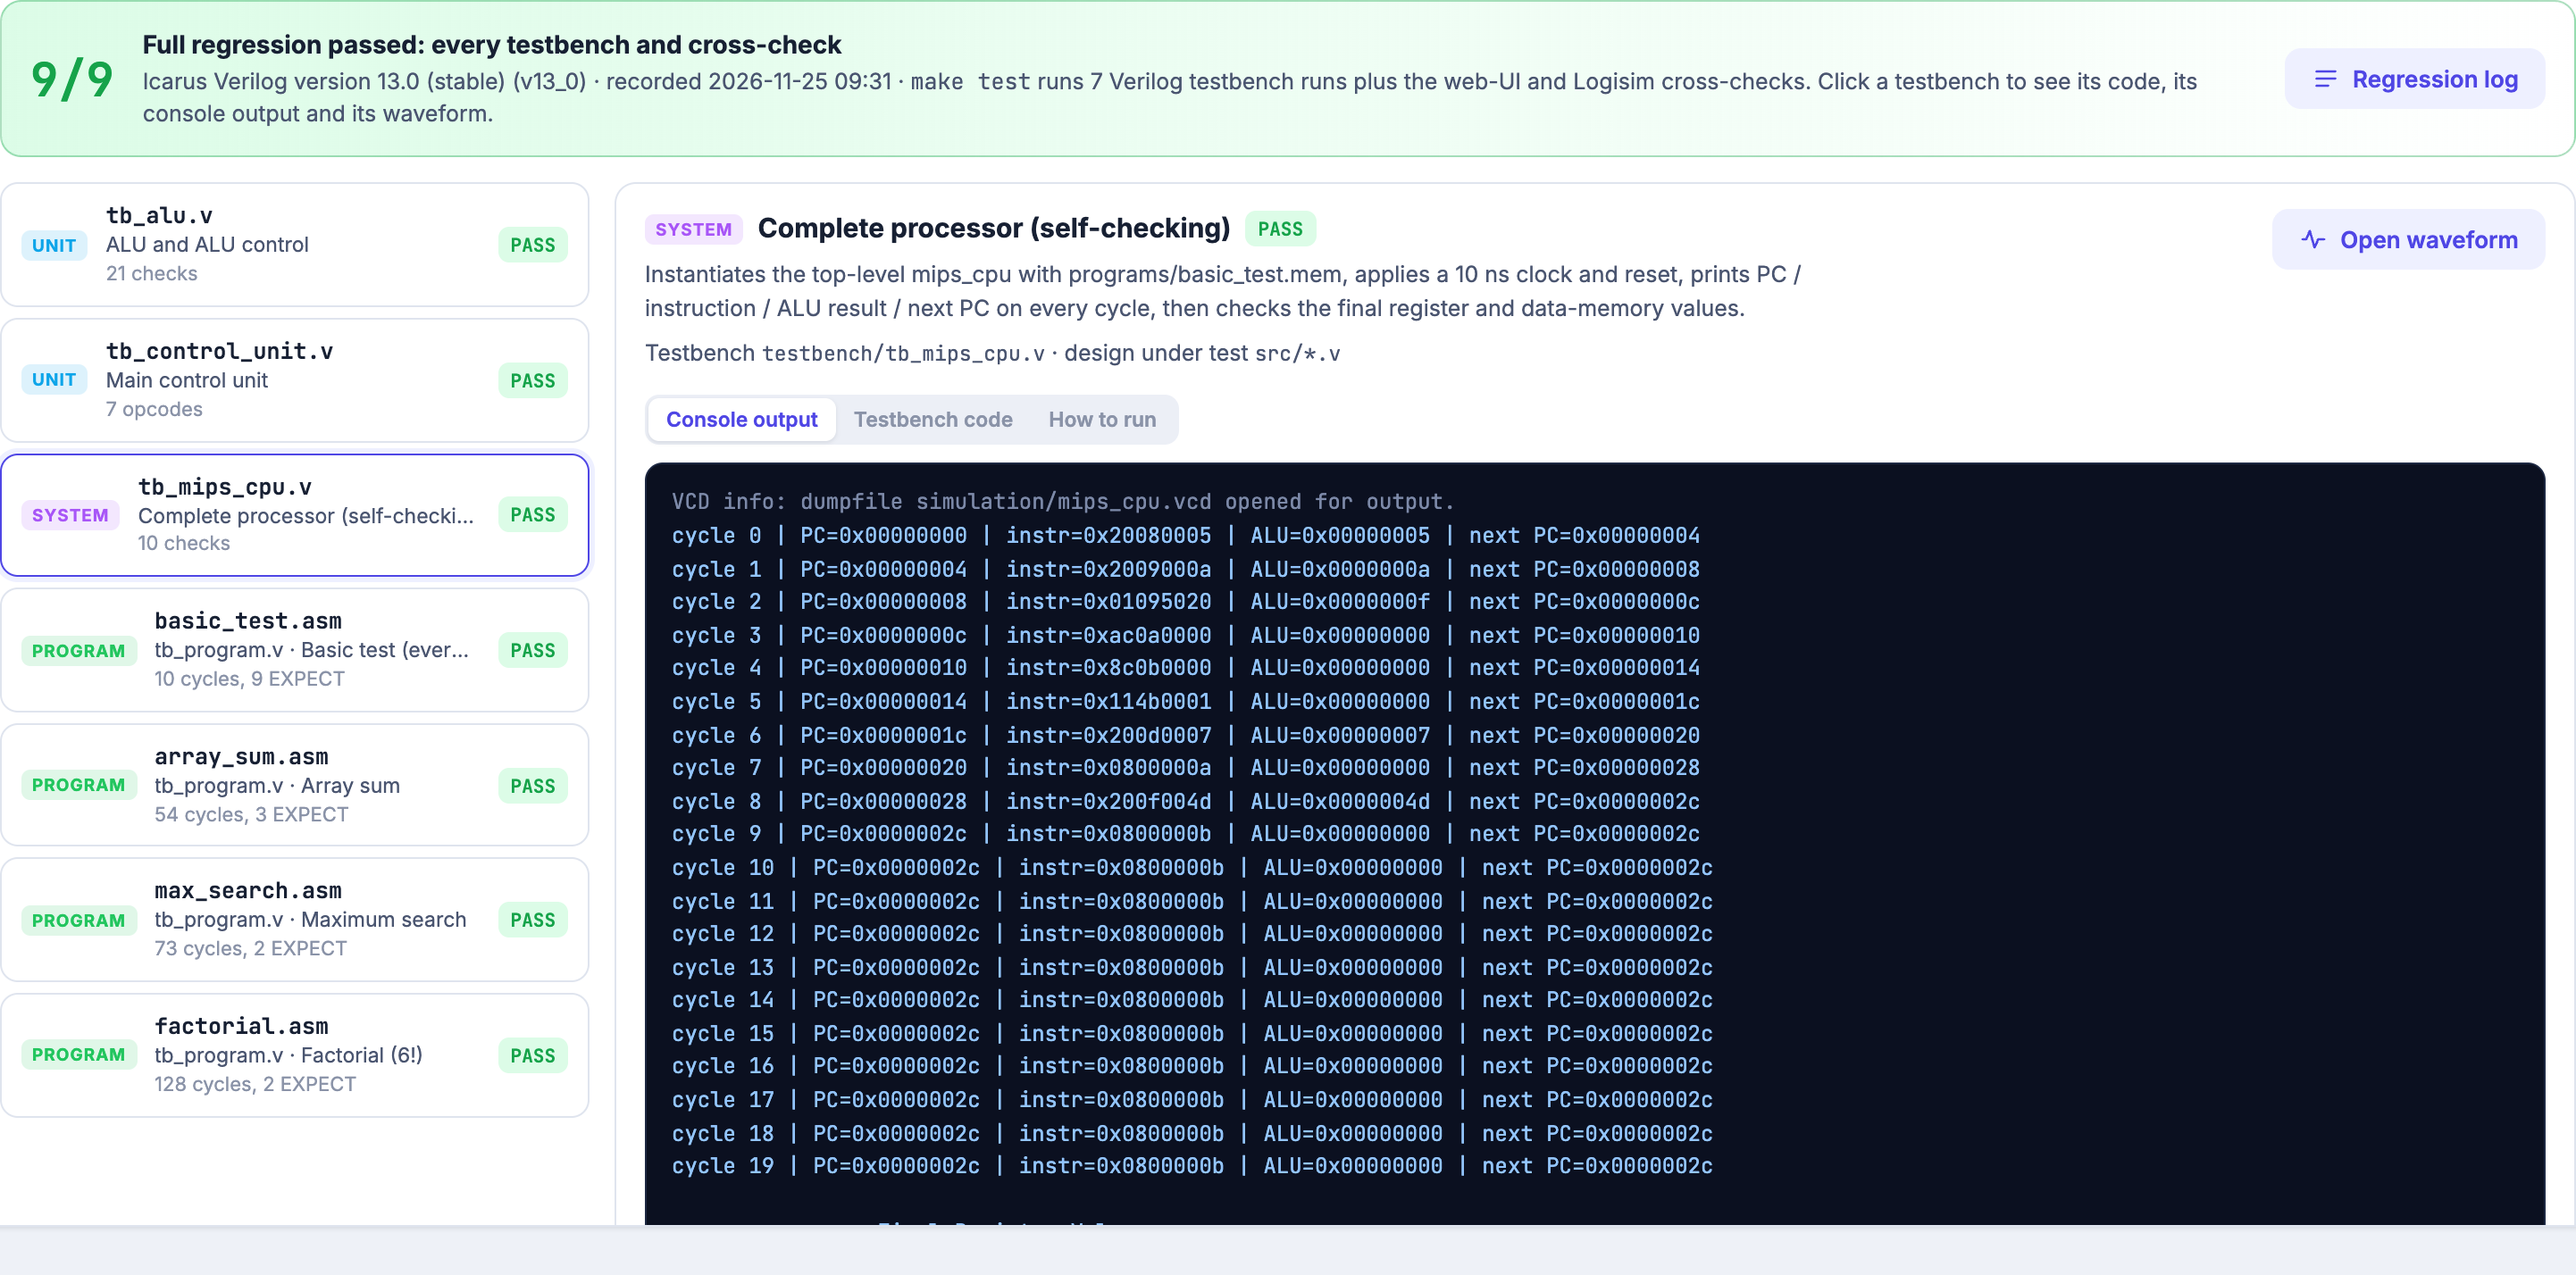
\includegraphics[width=\columnwidth]{testbench_tab.png}
\caption{Testbench tab of the web simulator: every testbench with its result, description, source code and the console output recorded from Icarus Verilog (here \texttt{tb\_mips\_cpu.v}).}
\label{fig:tbtab}
\end{figure}

\section{Results and Discussion}
\subsection{Demonstration Programs}
The basic test exercises every instruction class and ends with \$t7 = 77 and memory word 0 = 15. The array-sum program adds eight signed words and stores 110. The maximum-search program scans ten values with SLT and BEQ and finds 92. The factorial program computes 6! = 720 using multiplication by repeated addition. Together the programs exercise register arithmetic, immediate arithmetic, memory access, signed comparison, conditional branching and jumps, and every program runs with a CPI of exactly 1.

\subsection{Synthesis Results}
\label{sec:synth}
The design was synthesized with Yosys 0.71~\cite{yosys}. The technology-independent \texttt{mips\_core} contains 4,795 generic cells and 1,056 flip-flops after flattening and optimization; the flip-flops are dominated by the 32$\times$32-bit register file. The longest combinational path is 87 gate levels, running from the register-file read multiplexers through the ALU and branch adder to the next-PC and write-back logic. This illustrates the timing limitation of a single-cycle design: the slowest instruction path, which is LW (fetch, register read, address calculation, memory read and write-back), determines the clock period.

For a Xilinx Artix-7 target the complete system uses the resources in Table~\ref{tab:fpga}, which is below 2\% of the LUTs of an XC7A35T device. Yosys does not report timing in nanoseconds, so a maximum clock frequency requires device-specific timing analysis (for example in Vivado).

\begin{table}[t]
\caption{Artix-7 Synthesis Resource Use (Yosys 0.71)}
\label{tab:fpga}
\centering\footnotesize
\begin{tabular}{@{}lrl@{}}
\toprule
Resource & Used & Implementation role\\
\midrule
LUTs & 369 & Control, ALU, muxes, program ROM\\
CARRY4 & 35 & Adders (ALU, PC+4, branch target)\\
Flip-flops & 48 & PC and memory-port registers\\
RAM32M & 12 & Register-file storage\\
RAM256X1S & 32 & Data memory\\
MUXF7 & 1 & Multiplexer\\
\bottomrule
\end{tabular}
\end{table}

\subsection{Design Limitations}
The implementation is an educational subset rather than a complete MIPS32 processor. It does not implement exceptions, overflow detection, delay slots or pipelining. Memory accesses are word-aligned; the low two address bits are ignored and the address space wraps at 256 words. Unsupported opcodes behave as no-operations. Reset is synchronous and active-high and resets only the PC; registers and memories are initialized at start-up. Future work could add pipelining with hazard handling, exception support, a broader instruction set and device-specific timing analysis.

\section{Team Details and Contribution}
The five team members and their contributions are listed in Table~\ref{tab:team}. Although each member led one area, all members can explain the complete datapath, instruction formats, control signals, memory interface and verification approach.

\begin{table}[t]
\caption{Team Members and Contributions}
\label{tab:team}
\centering\footnotesize\setlength{\tabcolsep}{3pt}
\begin{tabular}{@{}p{1.7cm}p{1.45cm}p{4.5cm}@{}}
\toprule
Member & Enrollment & Contribution\\
\midrule
Avneet Singh & 2401010117 & ALU, ALU control, sign extension, datapath and instruction execution; assembler and sample programs\\
Khushi & 2401010225 & Processor architecture and Logisim-evolution circuit\\
Manpreet Singh & 2401010263 & Interactive web simulator (testbench and waveform views), project report and video\\
Riya Yadav & 2401010390 & Data and instruction memory, branch and jump logic; testbenches, regression and waveforms\\
Satvik Prasad & 2401020055 & Processor modules and RTL implementation (top level, core, control unit, register file, PC); synthesis\\
\bottomrule
\end{tabular}
\end{table}

\section{Conclusion}
A modular 32-bit single-cycle MIPS processor has been designed in Verilog-2001 and verified by simulation. The design separates the datapath and control logic from the instruction and data memories and supports a focused subset of arithmetic, logical, load/store, branch and jump instructions. Unit, system and program testbenches simulated with Icarus Verilog pass all checks, every one of the 265 simulated clock cycles matches an independent golden model, and the VCD waveforms show the expected control-signal and datapath activity for each instruction class. Synthesis shows a small Artix-7 footprint, while the 87-level critical path demonstrates the timing cost of a single-cycle architecture and motivates pipelining as the next step.

\appendices
\section{Instruction Execution Details}
\emph{R-type:} the control unit recognizes opcode 000000. The register file reads rs and rt, RegDst selects rd, ALUSrc selects the second register, and ALU control decodes the funct field into ADD, SUB, AND, OR or signed SLT. The result is written to rd.

\emph{ADDI:} the 16-bit immediate is sign-extended and selected as the second ALU operand. The sum is written to rt; negative immediates are preserved by sign extension.

\emph{LW and SW:} both compute the effective address as base register plus sign-extended offset. For LW, MemRead is asserted and MemtoReg selects the memory data for write-back to rt. For SW, rt is routed to the memory write-data input and MemWrite is asserted; no register is written.

\emph{BEQ:} the ALU subtracts rt from rs. If they are equal the zero flag is asserted, and Branch AND Zero selects PC+4 plus the shifted offset; otherwise execution continues at PC+4.

\emph{J:} the jump target is formed from the upper four bits of PC+4, the 26-bit target field and two zero bits. The jump path has priority over the branch path.

\section{Reproducing the Results}
All results in this report are produced by scripts in the repository, run from its root with Icarus Verilog, Python 3 and Yosys installed:
\begin{lstlisting}
make test                      # full regression (all testbenches)
make sim  PROG=array_sum       # one program: trace + VCD in simulation/
make wave PROG=array_sum       # timing diagram in docs/waveforms/
make synth                     # Yosys synthesis reports
python3 tools/export_sim_results.py   # testbench logs + VCDs for the web UI
\end{lstlisting}
The VCD files in \texttt{simulation/} can also be opened in GTKWave or in the web simulator's Waveform tab.


\begin{thebibliography}{9}
\bibitem{patterson} D. A. Patterson and J. L. Hennessy, \emph{Computer Organization and Design: The Hardware/Software Interface}, 5th ed. Waltham, MA, USA: Morgan Kaufmann, 2014.
\bibitem{mips32} MIPS Technologies, \emph{MIPS32 Architecture for Programmers, Volume II: The MIPS32 Instruction Set}, Rev. 2.00, 2003.
\bibitem{verilog} \emph{IEEE Standard for Verilog Hardware Description Language}, IEEE Std 1364-2005, 2006.
\bibitem{iverilog} S. Williams, ``Icarus Verilog,'' project documentation. [Online]. Available: \url{https://steveicarus.github.io/iverilog/}
\bibitem{yosys} YosysHQ, ``Yosys Open SYnthesis Suite: Documentation.'' [Online]. Available: \url{https://yosyshq.readthedocs.io/}
\bibitem{logisim} Logisim-evolution, ``Logisim-evolution documentation and project.'' [Online]. Available: \url{https://github.com/logisim-evolution/logisim-evolution}
\bibitem{bhardwaj} P. Bhardwaj, ``Design and simulation of a 32-bit RISC based MIPS processor using Verilog,'' \emph{Int. J. Res. Eng. Technol.}, vol. 5, no. 11, pp. 166--172, 2016.
\bibitem{phanindra} K. Phanindra, ``32-bit MIPS RISC processor,'' \emph{Int. J. Res. Appl. Sci. Eng. Technol.}, vol. 5, no. 10, pp. 1119--1123, 2017.
\bibitem{alsudany} S. M. Al-Sudany, A. S. Al-Araji, and B. M. Saeed, ``FPGA-based multi-core MIPS processor design,'' \emph{Iraqi J. Comput. Commun. Control Syst. Eng.}, vol. 21, no. 2, 2021, doi: 10.33103/uot.ijccce.21.2.2.
\end{thebibliography}

\end{document}
